\chapter{Desorption dynamics of RbHe exciplexes}\label{ch:rbhe-exciplexe}
	\lettrine[lines=4]{\color{activeColor}H}{ow} do we resolve the discrepancy between the experimental observation that Rb atoms, excited to the 5p$\,^2\Pi_{3/2}$ state, detach from the droplet surface, and TD-DFT simulations that show that they result in a surface-bound state? That is the question that led to this work. Upon photo-excitation of Rb to the 5p$\,^2\Pi_{3/2}$ state, a He atom may be attached to it forming a HeRb exciplex; this cannot happen if Rb is excited to the 5p$\,^2\Pi_{1/2}$ state because it finds a barrier (see \fig{fig:potentials}) preventing exciplex formation.

	In the gas phase, a HeRb 5p$\,^2\Pi_{1/2}$ exciplex can be formed if there is enough kinetic energy for Rb* to overcome the potential barrier; alternatively, the collision of the HeRb 5p$\,^2\Pi_{3/2}$ exciplex with another atom or complex might relax the Rb* atom from the 5p$\,^2\Pi_{3/2}$ to the 5p$\,^2\Pi_{1/2}$ state, overcoming the barrier as the potential wells for both states are at similar Rb-He distances. In the condensed (droplet) phase at 0.4 K temperature, neither of these mechanisms are available to explain the formation of HeRb 5p$\,^2\Pi_{1/2}$ exciplexes and their potential ejection.

	However, another possible way for this to happen is non-radiative de-excitation from the 5p$\,^2\Pi_{3/2}$ to the 5p$\,^2\Pi_{1/2}$ that populates the latter state and leaves the Rb* atom with enough kinetic energy so as to be ejected. Notice from \fig{fig:potentials} that the minimum of the 5p$\,^2\Pi_{3/2}$ potential is 12683 cm$^{-1}$, and that of the 5p$\,^2\Pi_{1/2}$ potential is at 12518 cm$^{-1}$; the value of this potential at the barrier is 12611 cm$^{-1}$. Thus, non-radiative de-excitation of the Rb* atom may add to its original kinetic energy of up to 165 cm$^{-1}$. It is worth noting that it will be ejected in the 5p$\,^2\Pi_{1/2}$ state, and not in the 5p$\,^2\Pi_{3/2}$ it was previously photo-excited to.

	This publication contains a extension of our combined experimental and theoretical investigation presented in the previous section. Here we focus on the formation of free RbHe-exciplex molecules from laser-excited Rb-doped He nanodroplets through the mechanism of electronic spin relaxation.% The role of relaxation of internal degrees of freedom of the RbHe exciplex in the desorption process has not been explicitly addressed.

	\begin{figure}
		\begin{center}
			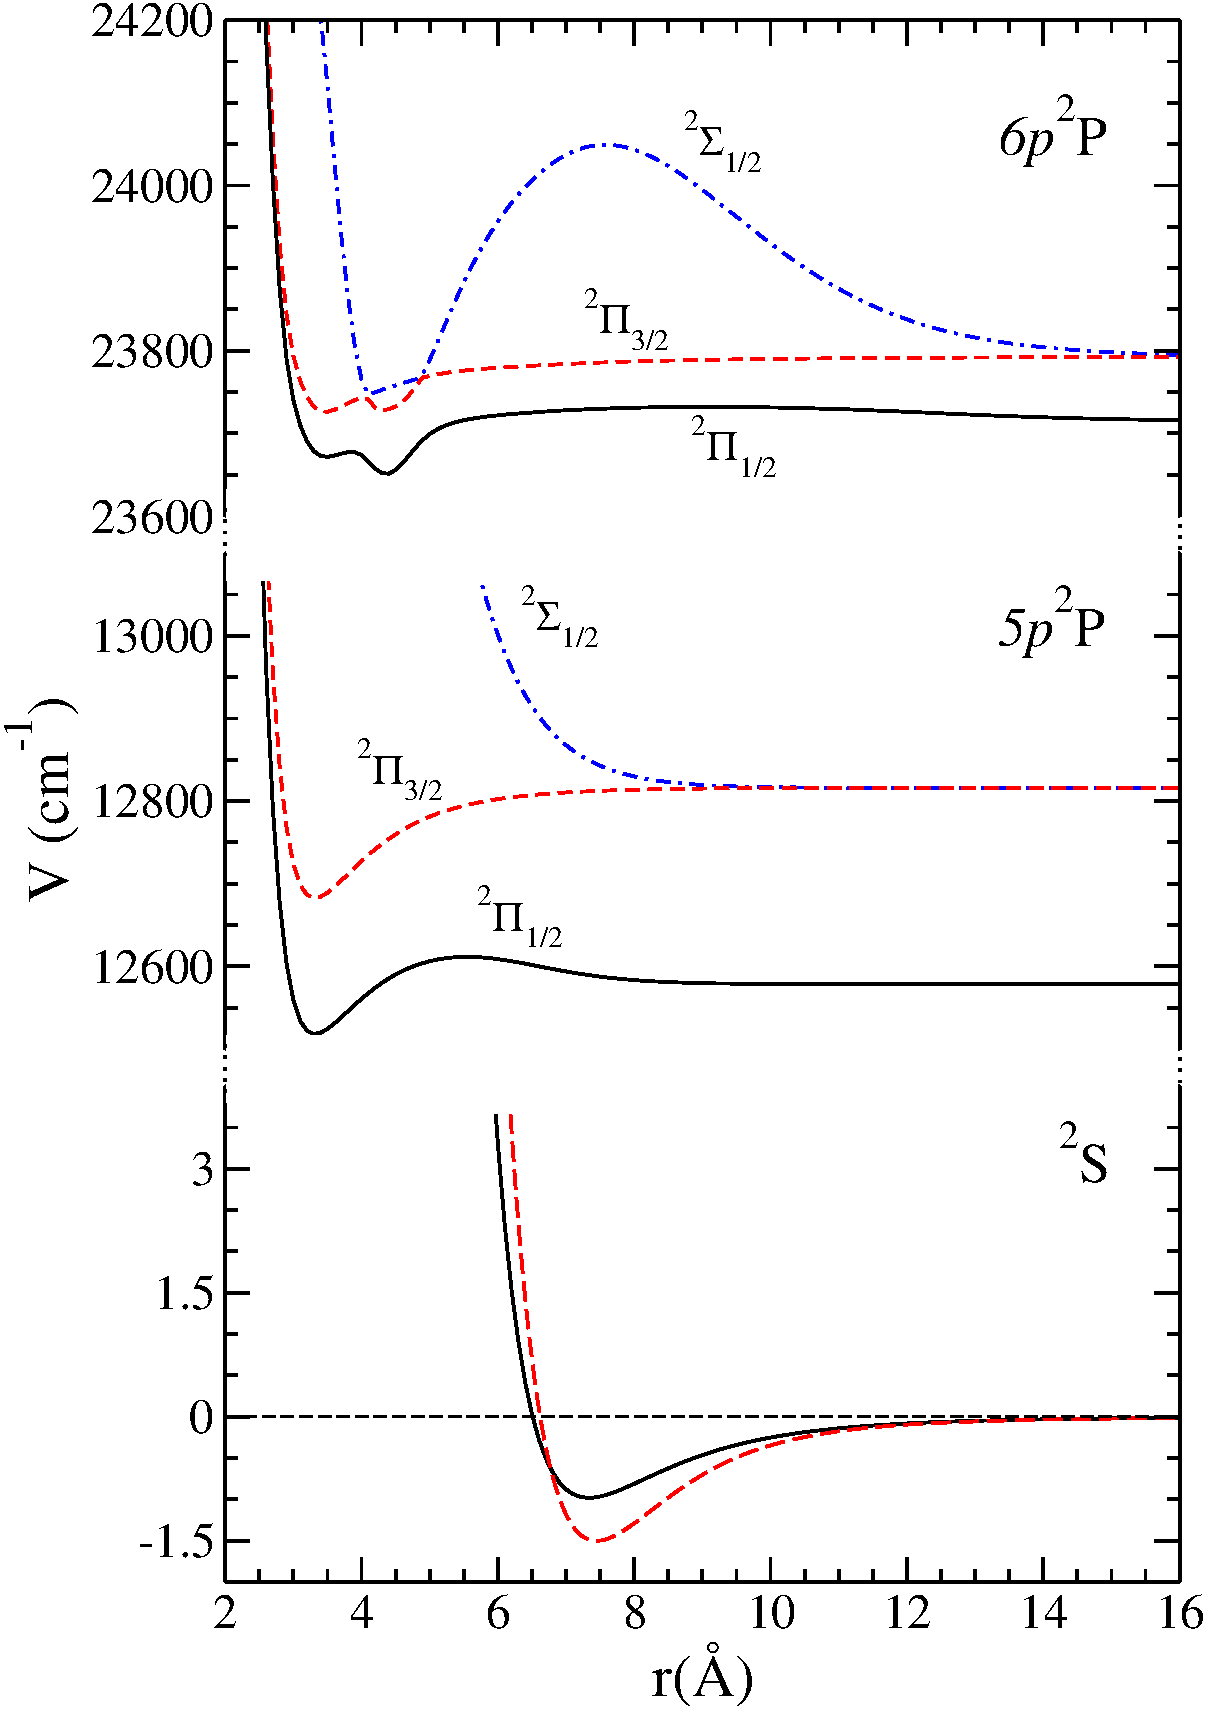
\includegraphics[width=\textwidth]{potentials}
		\end{center}
		\caption{$^2$S, 5p$\,^2$P, and 6p$\,^2$P Rb-He pair potentials used in this work. The splitting introduced by the spin-orbit interaction has been included. The $^2$S He-Rb pair potential of\rf{Pas83} is also displayed (bottom dashed line).}
		\label{fig:potentials}
	\end{figure}

	\cleardoublepage
	
%	\includepdf[pages={-}, scale=0.8, pagecommand={}]{pccp_vol20_no14_pp9309-9320.pdf}
	\includepdf[pages={-}, scale=0.9, pagecommand={}]{pccp_vol20_no14_pp9309-9320.pdf}